\documentclass[12pt]{article}
\usepackage[top=1in,bottom=1in,left=0.5in]{geometry}
\usepackage{graphicx}
\usepackage{amsfonts}
\usepackage{amsmath}

\DeclareMathOperator*{\argmin}{\arg\!\min}

\title{Shadow interpolation on images project}
\author{}
\date{2017}
\begin{document}
\maketitle



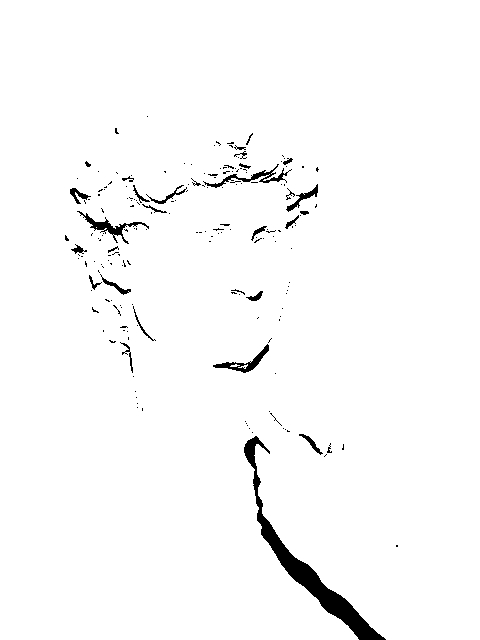
\includegraphics[scale=0.18]{a.jpg}
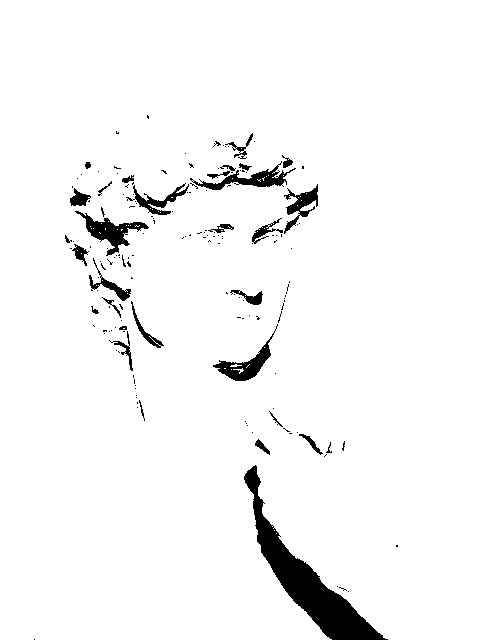
\includegraphics[scale=0.18]{b.jpg}
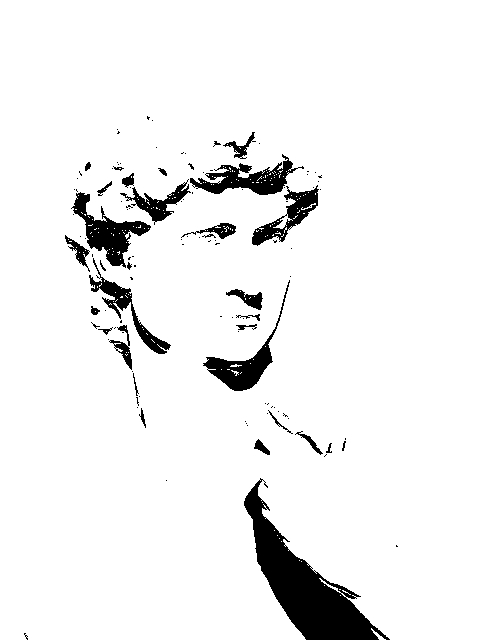
\includegraphics[scale=0.18]{c.jpg}
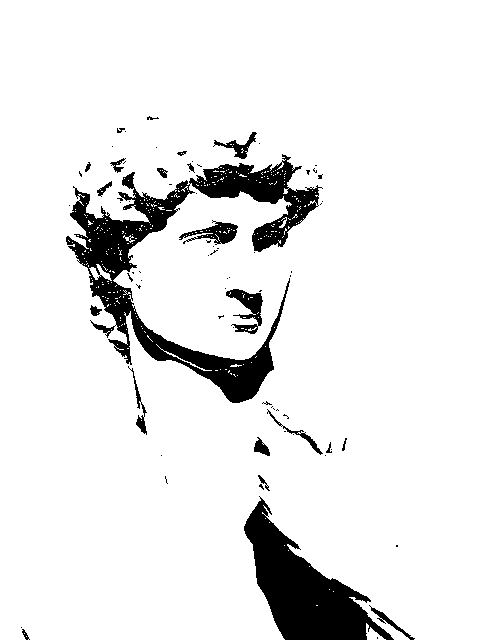
\includegraphics[scale=0.18]{d.jpg}
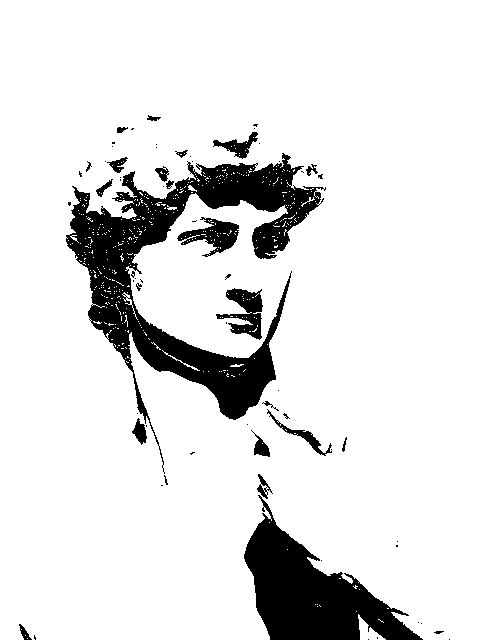
\includegraphics[scale=0.18]{e.jpg}

\section{problem statement}	
We are given a sequence of pictures of a diffusive object with various lighting conditions. \\
We know that in diffusive object, there are 3 basis functions that span all the possible pictures (determined by lighting direction). \\
And we would like to add shadows to this problem. the problem with shadows is that it can not be represented by a low amount of basis functions. \\
So we are seeking a smart interpolation for the representation of the missing parts between the images.

\newpage

\section{Simple interpolation }
\subsection{Definitions}
Given 2 pictures of logical shadow representation $I_0$ and $I_1$ where
$I_i \in \left\{ 0,1 \right\} ^ {H \times W}$ \\
$I_i$ is the shadow representation of image i. \\
We are seeking a vector mapping $$\Phi _v(t):\mathbb{R}^2\rightarrow\mathbb{R}^2$$
  $$ x\mapsto\Phi _v(t;x)$$
  With the constraints
$$\Phi _v(0) = id$$
$$I_1=I_0\cdot\Phi _v(1)$$
As an initial idea we will define $\Phi _v$ as 
$$\Phi _v = id + t \cdot v$$
This is just an initial model for the vector field and it is going to be changed when we advance with the project.
\\
\\
We define our discrete domain as a graph: $D:=(\nu,\varepsilon,f)$ \\
Where $\nu$ is set of image vertices (pixel corner) \\
$\varepsilon$ as the edges
and $f$ is image faces (pixel center)
\\
Using this definition, assuming there are $n$ vertices and $m$ faces, we define

\begin{center}
Image $I:\nu \rightarrow \mathbb{R} ,\ I \in \mathbb{R}^n $ \\
Vector field velocity $v:f \rightarrow \mathbb{R}^2 ,\ v \in \mathbb{R}^{2m} $
\end{center}

We want to calculate $\phi_v$ by minimizing 
$$ \argmin _v {\|I_1 - I_0 \cdot \Phi _v(1) \|}^2_D =
	\int \limits_D {\|I_1(x) - I_0(x) \cdot \Phi _v(1;x) \|}^2_D dx
$$
\\
This is an ill-posed problem, so we define a regularizing term as follows
$$ \displaystyle{ \int \limits_D \langle v, (id + \alpha \triangle) v \rangle da } $$
where $\alpha$ is constant
\\

\newpage
\textbf{Calculating the regularization term in matrix form:}
\begin{eqnarray}
\int \limits_D \langle v, (id + \alpha \triangle) v \rangle da &=& \\
\sum \limits_{j \in f} A_f(j) \cdot v(j)^T \cdot (id + \alpha \triangle) v(j) &=& \\
v^T \cdot A_f \cdot (id + \alpha \triangle) v
\end{eqnarray}
Where $A_f$ is a diagonal matrix of vertices areas. \\

\textbf{Calculating the data fidelity term in matrix form:}
\begin{eqnarray}
\int \limits_D {\|I_1 - I_0 \cdot \Phi _v(1) \|}^2_D \ da \\
\sum \limits_{i \in v} A_v(i) \cdot {\left(I_1(i) - I_0(i) \cdot \Phi _v(1;i) \right)}^2
\end{eqnarray}
Assigning $ \Phi _v(1;i) $ for every i, we get $ \Phi _v(1;i) = id(i) - v(i) $
using bilinear interpolation from faces to vertices \\
Where $ \displaystyle{v(i) = \frac{\sum \limits_{j \in N(i)} v(j)}{\sum \limits_{j \in N(i)} 1}} $  \\
is the mean value of the 1-ring of vertex i.
\begin{eqnarray}
\sum \limits_{i \in v} A_v(i) \cdot {\left[I_1(i) - I_0(i) \cdot \phi) \right]}^2 \\
\end{eqnarray}

We define functional map
$$ C[\phi] = Id + t \cdot D[v] $$
Where D is an operator on image $I$ defined as
$$ D[v] \cdot I = I_n^m \left\langle v , grad I \right \rangle $$
$I_n^m$ operator represent a matrix form of interpolation of vertices to faces
\\

The data fidelity term is
$$ (I_1 - C[\phi] I_0)^T A_v (I_1 - C[\phi] I_0)$$


\newpage
\subsection{Solution}
We define energy temp as sum of the data fidelity term and the regularization term

$$ E = (I_1 - C[\phi] I_0)^T A_v (I_1 - C[\phi] I_0) + (v^T \cdot A_f \cdot (id + \alpha \triangle) v) $$

We want to minimize it, so we will derive it as follows:

\textbf{1. Deriving the data fidelity term}
$$ - \left(  \frac{\partial C[\phi]}{\partial v} I_0  \right) ^T A_v (I_1 - C[\phi] I_0) +
(I_1 - C[\phi] I_0)^T A_v^T \left( - \frac{\partial C[\phi]}{\partial v} I_0  \right)
$$
$A_f$ is diagonal, so $A_f = A_f^T$

furthermore, both terms are scalars, so they are equal, because we can take the transpose of one of those terms.

We get
$$ -2 \left(  \frac{\partial C[\phi]}{\partial v} I_0  \right) ^T A_v (I_1 - C[\phi] I_0) $$

* We will derive $C[\phi]$ later..
\\


\textbf{2. Deriving the regularization term}
$$
\left(
\frac{\partial v}{\partial v}
\right) ^T
A_f (Id + \alpha \triangle) v +
\left(
\frac{\partial v}{\partial v}
\right) ^T
(Id + \alpha \triangle)^T A_f^T v 
$$
Notice that $ A_f (Id + \alpha \triangle) $ is symmetric, because its components are symmetric.
Therefore, we can take its transpose in one of the components.
$$ 
2 \left(
\frac{\partial v}{\partial v}
\right) ^T
A_f (Id + \alpha \triangle) v
$$
\\

By combining both derivatives, we get
$$ \frac{\partial E}{\partial v} =
-2 \left(  \frac{\partial C[\phi]}{\partial v} I_0  \right) ^T A_v (I_1 - C[\phi] I_0)
+
2 \left(
\frac{\partial v}{\partial v}
\right) ^T
A_f (Id + \alpha \triangle) v
$$

And the solution is simply given by steepest descent process
$$ v^{k+1} = v^k - \gamma
\frac{\partial E}{\partial v}
$$

\newpage
\textbf{Derivative of $C[\phi]$}

$C[\phi]$ was defined as
$$ C[\phi] I = I + t \cdot D[v] I $$
derivative
$$ \frac{\partial C[\phi] I}{\partial v} =
$$
$$
\frac{\partial}{\partial v}
\left(
I + t \cdot D[v] I
\right) =
$$
$$
t \frac{\partial}{\partial v}
\left(
D[v] I
\right) =
$$
$$
t \frac{\partial}{\partial v}
\left(
I_n^m \left\langle v , grad I \right \rangle
\right)
$$
* Inner product of 2 vector fields can be represented as a matrix form as follows

let be 2 vector fields $u$ and $v$. their inner product
$$ \left\langle
v,u
\right\rangle = [v]u = [u]v $$
Where [v] = $
\left[
\begin{array}{cccc}
v_{1_x} & 0...0 & v_{1_y} & 0...0 \\ 
v_{2_x} & 0...0 & v_{2_y} & 0...0 \\ 
\vdots & \vdots & \vdots & \vdots \\ 
v_{m_x} & 0...0 & v_{m_y} & 0...0
\end{array}
\right]
$

and the second vector field is represented as a column vector of $ 
u = \left[
\begin{array}{c}
u_{1_x} \\ 
\vdots \\ 
u_{m_x} \\ 
u_{1_y} \\ 
\vdots \\ 
u_{m_y}
\end{array} 
\right]
$


Back to our derivation of the term, we get
$$
t \frac{\partial}{\partial v}
\left(
I_n^m \left\langle v , grad I \right \rangle
\right) =
$$
$$
t I_n^m \frac{\partial}{\partial v}
\left(
\left[ grad I \right] v
\right) =
$$
$$
t I_n^m
\left[ grad I \right]
\frac{\partial v}{\partial v}
$$

Thus, the derivative of the energy term is
$$
\frac{\partial E}{\partial v} =
- 2 t
\left[
grad I_0
\right]^T
(I_n^m)^T
A_v
(I_1 -C[\phi] I_0)
+ 2 A_f (Id + \alpha \triangle)v
$$








\end{document}